%%%%%%%%%%%%%%%%%%%%%%%%%%
\chapter{Background}
\label{ch:background}
This chapter focuses on the introduction of preliminary concepts necessary to understand the general approach, as well as the utilities chosen in our implementation.
%%%%%%%%%%%%%%%%%%%%%%%%%%%%%%%%%%%%%%%%%%%%%%%%%%%%%%%%%%%%%%%%%%%%%%%%%%%%%%%%%%%%%%%%%%%%%%%%%%%%%%%%%%%%%%%%%%%%%%%%%%%%%%%%%%%%%%%%%%%%%%%%%%%%%%%%%%%%

\section{General approach}
\label{sec:2background:approach}
Our approach utilizes pure Bayesian statistics wherever possible. We develop a probabilistic model for an observable EEG time series, and then incorporate weak supervision through the use of a domain-specific prior. Our algorithm, Bayesian Seizure Likelihood Estimation (BSLE), performs inference computations with the developed model, to assess the likelihood of an upcoming seizure. The output is tested and evaluated for model fit and predictive capabilities.

%%%%%%%%%%%%%%%%%%%%%%%%%%%%%%%%%%%%%%%%%%%%%%%%%%%%%%%%%%%%%%%%%%%%%%%%%%%%%%%%%%%%%%%%%%%%%%%%%%%%%%%%

% Lower the section header to match the (very) long chapter header
% \renewcommand*\sectionmarkformat{\\ \autodot\thesection\enskip}
%%%%%%%%%%%%%%%%%%%%%%%%%%


% \renewcommand*\sectionmarkformat{\autodot\thesection\enskip}
%%%%%%%%%%%%%%%%%%%%%%%%%%

%%%%%%%%%%%%%%%%%%%%%%%%%%%%%%%%%%%%%%%%%%%%%%%%%%%%%%%%%%%%%%%%%%%%%%%%%%%%%%%%%%%%%%%%%%%%%%%%%%%%%%%%%%%%%%%%%%%%%%%%%%%%%%%%%%
\section{Problem setup}
\label{sec:2background:setup}
Consider the problem of modeling the relationship between EEG signals ($E$) from the epileptic brain, the occurrence of seizures ($S$), and an external stream of timestamps denoting seizure events, commonly provided by expert annotators ($A$), throughout time ($T$).

Specifically, we are given a dataset $D = \{e_t, a_t\}_{t_0}^{t_f}$ where $e_t \in \mathbb{R}^{c \times \tau}$ is the observed EEG segment with $c$-channels of duration $\tau$ recorded at time $t$, and $a_t \in \{0, 1\}$ is a clinically-approved annotation denoting whether or not a seizure event began within the time-window $[t, t + \tau ]$.

We wish to construct a model for $\prob[S, E, t]$, and then apply it with Bayes' rule to infer the likelihood of a seizure at time $t$:

\begin{equation}
prob[S \mid E, t] \propto \prob[E \mid S, t] \prob[S \mid t]
\end{equation}

It should be evident that this procedure is general in that each component on the \rhs can be estimated independently. We hope that future attempts at seizure likelihood estimation will utilize our Bayesian by incorporating new likelihood functions and priors.

%%%%%%%%%%%%%%%%%%%%%%%%%%%%%%%%%%%%%%%%%%%%%%%%%%%%%%%%%%%%%%%%%%%%%%%%%%%%%%%%%%%%%%%%%%%%%%%%%%%%%%%%
\section{Circadian distributions}
\NS[inline]{write about circadian distributions}

%%%%%%%%%%%%%%%%%%%%%%%%%%%%%%%%%%%%%%%%%%%%%%%%%%%%%%%%%%%%%%%%%%%%%%%%%%%%%%%%%%%%%%%%%%%%%%%%%%%%%%%%

\section{Inhomogeneous Poisson processes}
\NS[inline]{write about Cox process}


%%%%%%%%%%%%%%%%%%%%%%%%%%%%%%%%%%%%%%%%%%%%%%%%%%%%%%%%%%%%%%%%%%%%%%%%%%%%%%%%%%%%%%%%%%%%%%%%%%%%%%%%

\section{Hierarchical Time Series Modeling}
\NS[inline]{write about multilevel modeling of EEG time series}


%%%%%%%%%%%%%%%%%%%%%%%%%%%%%%%%%%%%%%%%%%%%%%%%%%%%%%%%%%%%%%%%%%%%%%%%%%%%%%%%%%%%%%%%%%%%%%%%%%%%%%%%%%%%%%%%%%%%%%%%%%%%%%%%%%

\subsection{Gaussian processes}
\label{sec:2background:GPs}
A Gaussian process (GP) \cite{rasmussen2006cki} is \emph{a collection of random variables, any finite number of which have a joint Gaussian distribution}.

A Gaussian process $f(x)$ is fully specified by a mean function $\mu(x)$ and a covariance function, or a kernel, $k(x,x')$, by-way-of:

\begin{align}
    m(x) &= \E[f(x)] \\
k(x,x') &= \E[(f(x)-m(x))(f(x')-m(x')]
\end{align}

And it is denoted:

\begin{align}
    f(x) \sim \mathcal{GP}(m(x), k(x,x'))
\end{align}

In this work we will take the mean function to be zero.

\subsubsection{parameter estimation (inference)}
Gaussian processes are commonly used for time series modeling with machine learning. To see why this makes sense, imagine the input $x$ is the time point, and the output $f(x)$ is the time series value at time $x$. Computationally, this is feasible because the function's values are estimated only at a finite number of points of interest.
Using optimization techniques, the model's hyperparameters are inferred to match observed data by maximizing the likelihood function $p(f(x) \mid \Vec{\theta})$ (termed maximum likelihood estimation, or MLE). The learned hyperparameters capture global evolutionary dynamics of the time series (see figure \ref{fig:3methods:posterior_draws} in the Methods section).

\subsubsection{The Matérn class of covariance functions}
The Matérn class of covariance functions is given by:

\begin{align}
    k_{Matern}(x,x') = \frac{2^{(1-\nu)}}{\Gamma(\nu)}(\sqrt{2\nu}d)^\nu K_\nu (\sqrt{2\nu}d)
\end{align}

Where:
\begin{itemize}
    \item $d = (x-x')^T \Phi^{-2} (x - x')$ is the distance between $x$ and $x'$ scaled by the \emph{lengthscale} parameter $\Phi$.
    \item $\nu$ is a smoothness parameter. In this work, it is taken to be $\frac{3}{2}$.
    \item $K_\nu$ is a modified Bessel function.
\end{itemize}

\subsubsection{Multitask Gaussian processes}
In case $f(x)$ is a vector function, multiple output functions are modeled in conjunction for the same input values, so-called multitask Gaussian process modeling. In this case, given inputs $x$ and $x'$, and tasks $i$ and $j$, the covariance between two datapoints and two tasks is given by:

\begin{align}
\label{eq:2background:multitask}
    k([x,i], [x',j]) = k_{inputs}(x,x') \cdot k_{tasks}(i,j)
\end{align}

Where $k_{inputs}$ is a standard kernel (e.g., Matérn) that operates on the inputs, and $k_{tasks}$ is a lookup table containing inter-task covariance.

%%%%%%%%%%%%%%%%%%%%%%%%%%%%%%%%%%%%%%%%%%%%%%%%%%%%%%%%%%%%%%%%%%%%%%%%%%%%%%%%%%%%%%%%%%%%%%%%%%%%%%%%

\section{mixture models}
\NS[inline]{write about mixture models}

Gaussian mixture models \cite{theodoridis2015machine} are used to model the distribution of an unknown set of vectors $\{x\} \subseteq \mathbb{R}^l$ as a linear combination (i.e., a mixture) of different Gaussian distributions, that is,

\begin{align}
    p(x) = \sum_{k=1}^{K}p_kp(x \mid k; \zeta_k)
\end{align}

where $\{\zeta_k\}$ parametrize the individual Gaussian distributions:
\begin{align}
    p(x \mid k ; \zeta_k) = p(x \mid k; \mu_k, \sigma_k) = \mathcal{N}(x \ mid \mu_k, \sigma_k)
\end{align}

Fitting the model provides an approximation $\hat p(x \mid k; \zeta_k)$ of the dataset's underlying pdf.

\subsection{von Mises distribution}

The von Mises distribution is defined as:

\begin{align}
    f(x | \mu, \kappa ; \omega) = \frac{\exp (\kappa \cos (\omega (x - \mu)))}{2 \pi I_0(\kappa)}
    \label{eq:2background:vm_density}
\end{align}

Visually, the resulting distribution is similar to a bell-shaped normal distribution on a circle (see figure \ref{fig:2background:vm_density}). In the definition above, $\mu$ determines the center of the bell,  $\kappa$ the spread, and $\omega$ scales the period length. In this work, we set $\omega \gets \frac{2\pi}{24}$ to scale the period to 24-hours, and drop it from the notation for brevity in the following text.

\begin{figure}[htbp]
    \centering
    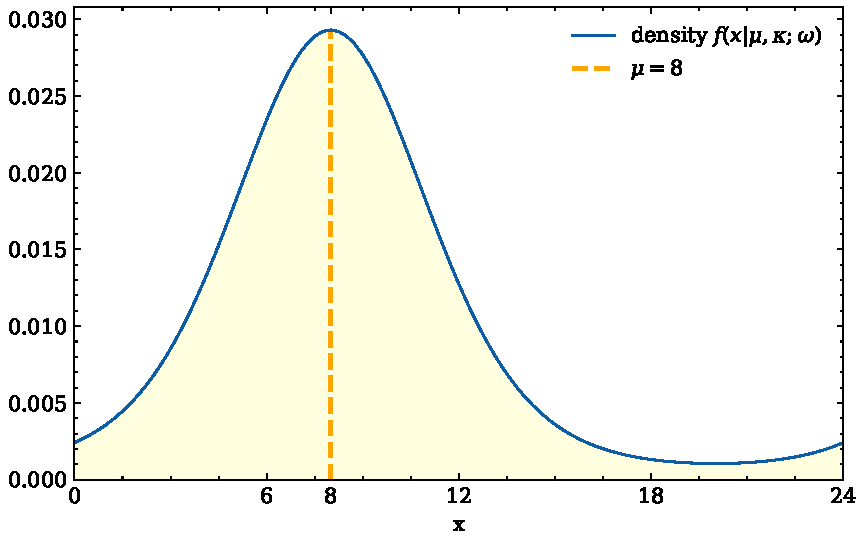
\includegraphics[width=\floatwidth]{02Background/Figs/VM/vm_density.pdf}
    \Caption{Von Mises distribution}{
	The von Mises distribution probability density function (also known as the circular normal distribution) for $\mu=8$, $k=1/0.6$, $\omega=\frac{2 \pi}{24}$
    }
    \label{fig:bsle:vm_density}
\end{figure}

\begin{figure}[htbp]
    \centering
    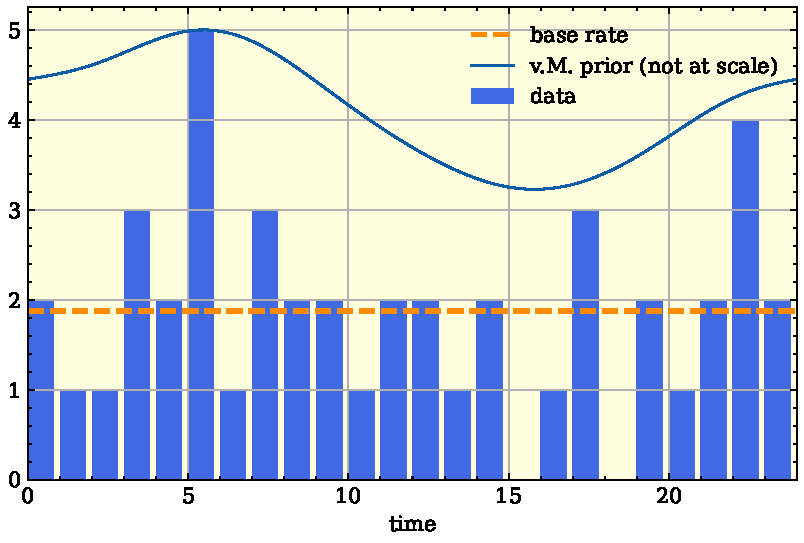
\includegraphics{5Results/figs/prior/vm_prior.pdf}
    \caption{non-normalized v.M. prior overlayed on empirical circadian seizure distribution for I004\_A0003\_D001}
    \label{fig:vm_prior}
\end{figure}



%%%%%%%%%%%%%%%%%%%%%%%%%%%%%%%%%%%%%%%%%%%%%%%%%%%%%%%%%%%%%%%%%%%%%%%%%%%%%%%%%%%%%%%%%%%%%%%%%%%%%%%%%%%%%%%%%%%%%%%%%%%%%%%%%%

\section{Model validation}
\NS[inline]{write about model validation}

\subsection{Bayesian model checking}
\NS[inline]{write about Bayesian model checking}

\subsection{Linear probing}
% https://arxiv.org/pdf/1610.01644.pdf
% https://arxiv.org/pdf/2002.05709.pdf
% https://www.youtube.com/watch?v=HJn-OTNLnoE
\NS[inline]{rewrite Linear probing section}
The \emph{support vector machine} (SVM) is a popular method for solving problems in classification, regression and novelty detection \cite{bishop2006pattern}. Fundamentally, it is a two-class linear classifier, i.e., it relies on linear models of the form

\begin{align}
    y(x) = w^T \phi(x) + b
\end{align}

where $\phi(x)$ denotes a fixed feature-space transformation, and $b$ is the bias parameter. The training data set comprises $N$ input vectors $x_1,..., x_N$, with corresponding target values $t_1, ..., t_N$, where $t_n \in \{-1, 1\}$, and new data points $x$ are classified according to the sign of $y(x)$.

By fitting the SVM to a training set and scoring the predictive accuracy on a hold-out test set, we can quantify the linear separability of the dataset. This is used as a proxy for representation quality.

%%%%%%%%%%%%%%%%%%%%%%%%%%%%%%%%%%%%%%%%%%%%%%%%%%%%%%%%%%%%%%%%%%%%%%%%%%%%%%%%%%%%%%%%%%%%%%%%%%%%%%%%%%%%%%%%%%%%%%%%%%%%%%%%%%

\section{Methods for evaluating forecast skill}
\NS[inline]{write about forecast skill evaluation methods}